\chapter{Introduction}

\section{Background}

The talk by Milanfar \cite{siam_slides_2016}, working at Google Research, about using the Graph Laplacian Operator for Image Processing purposes awakes curiosity.

Indeed, Milanfar reports that these techniques to build filters are used on smartphones, which means it is done in a reasonable time with limited computational resources.
Over 2 billion photos are shared daily on social media \cite{siam_slides_2016}, with very high resolutions and filters are often applied on them.

% Other filters problem, why we need this report and work here

\section{Objective}

The objective of this thesis is to, in a first place, understand and implement image processing algorithms shown by Milanfar's work on 2D images at Google.
We want to observe the performance and results of these algorithms to validate the usage of intrinsic spectral properties of an image.
For instance, the spectrum of the graph associated to an image can serve for image segmentation.
Applied in a fine-grained manner, this segmentation could lead to image compression.
More classic algorithm can also be achieved with the described approach, such as image denoising, deblurring, sharpening, etc.

The next step includes extending these techniques on 3D images.
Given the results, new scalable processing approaches for 3D images could be explored.
These also include standard processing filters such as denoising and sharpening, but also segmentation and compression techniques.

These approaches, even though faster than other filters, still require computations which can grow large in the 3D case.
That is why we want to apply the algorithm on high performance architectures in order to achieve reasonable computation times.
These will apply preconditioning our systems of linear equations with domain decomposition methods and use Krylov methods for solving.

\section{Related work}

\paragraph{}
We will explore three topics concerning this project.
First of all, we will have an overview of what spectral graph theory is about.
Then, we will dive into 2D image processing using the graph Laplacian operator, focusing three applications: denoising, sharpening and image segmentation.
For each of them, we show a classical algorithm, a newer spectral approach and then a short comparison of them.
Next, we present what has been done in 3D image processing so far using spectral graph theory, essentially using the graph Laplacian operator again.
Finally, we touch a few words on domain decomposition methods.

\subsection{Spectral graph theory}

\paragraph{}
Spectral graph theory has a long history starting with matrix theory and linear algebra that were used to analyse adjacency matrices of graphs.
It consists in studying the properties of graphs in relation to the eigenvalues and eigenvectors of the adjacency or Laplacian matrix.
The eigenvalues of such a matrix are called the spectrum of the graph.
The second-smallest eigenvalue has been called ``algebraic connectivity of a graph" by Fiedler \cite{fiedler_algebraic_1973}, and is therefore also known as \textit{Fiedler value}, because it contains interesting information about the graph.
Indeed, it can show if the graph is connected, and by extending this property, we can count the number of connected components in the graph through the eigenvalues of the graph Laplacian.

The field of spectral graph theory is very broad and the eigendecomposition of graphs is used in a lot of areas.
It was first applied in chemistry because eigenvalues can be associated with the stability of molecules.
Spectral graph theory has many other applications such as graph colouring, graph isomorphism testing, random walks and graph partitioning among others.

One of the most complete works about spectral graph theory is \cite{chung_spectral_1997} by Fan Chung.
This monograph exposes many properties of graphs, the power of the spectrum and how spectral graph theory links the discrete world with the continuous one.

\paragraph{Laplacian matrix}
Since the adjacency matrix of a graph only holds basic information about it, we usually augment it to the Laplacian matrix.
Multiple definitions of the Laplacian matrix are given in \cite{chung_spectral_1997} and \cite{siam_slides_2016}, and each one holds different properties.
The most common ones are the Normalised Laplacian and the Random Walk Laplacian.
However, more convenient formulations, like the ``Sinkhorn" Laplacian \cite{milanfar_symmetrizing_2013} and the Re-Normalised Laplacian \cite{siam_slides_2016}, have been proposed since.

\paragraph{The Spectral Theorem}
Some Laplacian definitions result in a real symmetric matrix, which is a property that is particularly interesting for spectral theory because of the Spectral Theorem \cite{zhang_spectral_2010}.
Let \(M\) be a real symmetric matrix of dimension \(n\), then
\[S = \Phi \Pi \Phi^T = \sum_{i=1}^n \lambda_i \phi_i \phi_i^T,\]
the eigendecomposition of \(S\) with \(\Phi = [\phi_1 \phi_2 \dots \phi_n ]\) the matrix of eigenvectors of \(S\) and \(\Pi\) the diagonal matrix of the eigenvalues of \(S\).
We note that the eigenvalues of \(S\) are real and that the eigenvectors are orthogonal, i.e., \(\Phi^T\Phi = I\), with \(I\) the identity matrix.

\paragraph{Cheeger's inequality}
One of the most fundamental theorems of spectral graph theory concerns the Cheeger's inequality and Cheeger constant.
It approximates the sparsest cut of a graph with the second eigenvalue of its Laplacian.

The Cheeger constant \cite{cheeger_lower_1969} measures the degree of ``bottleneck" of a graph, useful for constructing well-connected graphs.
Considering a graph \(G\) of \(n\) vertices, the Cheeger constant \(h\) is defined as
\[h(G) = min_{0 < |S| \le \frac{n}{2}} \frac{|\partial S|}{|S|},\]
where \(S\) is a subset of the vertices of \(G\) and \(\partial S\) is the \textit{edge boundary} of \(S\) to have all edges with exactly one endpoint in \(S\), or formally
\[\partial S = {{u, v} \in E(G) : u \in S, v \notin S},\]
with \(E(G)\) the edges of graph \(G\).

Cheeger's inequality defines a bound and relationship on the smallest positive eigenvalue of the Laplacian matrix \(\Lapl \) such as
\[\lambda_1(\Lapl) \ge \frac{h^2(\Lapl)}{4}.\]

When the graph \(G\) is \(d\)-regular, thanks to \cite{cvetkovic_spectra_1980}, we also have an inequality between \(h(G)\) and the second-smallest eigenvalue \(\lambda_2\) such as
\[\frac{1}{2}(d-\lambda_2) \le h(G) \le \sqrt{2d(d-\lambda_2)},\]
where \(d - \lambda_2\) is also called the \textit{spectral gap}.

\paragraph{}
The Laplacian is the foundation of the heat equation, fluid flow and essentially all diffusion equations.
It can generally be thought that the Laplacian operator is a center-surround average \cite{siam_slides_2016} of a given point.
Applying the graph Laplacian operator on an image provides useful information about it and enables possibilities of interesting image processing techniques.

\subsection{2D image processing}

\subsubsection{Denoising}

\paragraph{Background}
Even with high quality cameras, denoising and improving a taken picture remains important.
The two main issues that have to be addressed by denoising are blur and noise.
The effect of blur is internal to cameras since the number of samples of the continuous signal is limited and it has to hold the Shannon-Nyquist theorem \cite{buades_review_2005}.
Noise comes from the light acquisition system that fluctuates in relation to the amount of incoming photons.

To model these problems, we can formulate the deficient image as,
\[y = z + e,\]
where \(e\) is the noise vector of variance \(\sigma^2\), \(z\) the clean signal vector and \(y\) the noisy picture.

What we want is a high-performance denoiser, capable of scaling up in relation to increasing the image size and keeping reasonable performances.
The output image should come as close as possible to the clean image.
As an important matter, it is now accepted that images contain a lot of redundancy.
This means that, in a natural image, every small enough window has many similar windows in the same image.

\paragraph{Traditional, patch-based methods}
The image denoising algorithms review proposed by \cite{buades_review_2005} suggests that the NL-means algorithm, compared to other reviewed methods, comes closest to the original image when applied to a noisy image.
This algorithm takes advantage of the redundancy of natural images and for a given pixel i, predicts its value by using the pixels in its neighbourhood.

In \cite{dabov_image_2007}, the authors propose the BM3D algorithm, a denoising strategy based on grouping similar 2D fragments of the image into 3D data arrays. Then, collaborative filtering is performed on these groups and return 2D estimates of all grouped blocks.
This algorithm exposed state-of-the-art performance in terms of denoising at that time.
The results are still one of the best for a reasonable computational cost.

\paragraph{Global filter}
In the last couple of years, global image denoising filters came up, based on spectral decompositions \cite{glide_2014}.
This approach considers the image as a complete graph, where the filter value of each pixel is approximated by all pixels in the image.
We define the approximated clean image \(\hat{z}\) by,
\[\hat{z} = Wy,\]
where \(W\) is our data-dependent global filter, a \(n \times n\) matrix, \(n\) the number of pixels in the picture.
\(W\) is computed from the graph affinity matrix\footnote{Also called kernel matrix or similarity matrix} \(K\), also of size \(n \times n\), such as
\[K = {\mathcal{K}_{ij}},\]
where \(\mathcal{K}\) is a similarity function between two pixels \(i\) and \(j\).
As the size of \(K\) can grow very large, we must sample the image and compute an approximated \(\tilde{K}\) on this subset using the Nystr\"om extension.
Because \(K\) is symmetric, it can in fact be approximated through its eigenvalues and eigenvectors with
\[\tilde{K} = \phi_K \Pi_K \phi_K^T.\]
Knowing that the eigenvalues of \(K\) decay very fast \cite{siam_slides_2016}, the first eigenvectors of the subset of pixels are enough to compute the approximated \(\tilde{K}\).

Generally, as proposed in \cite{glide_2014} and \cite{talebi_asymptotic_2016}, to improve the denoising performance of global filters, pre-filtering techniques are used.
It is proposed to first apply a NL-means algorithm to the image to reduce the noise, but to still compute the global filter on the noisy input and apply the filter to the pre-filtered image.

\paragraph{Comparison between patch-based and global methods}
As \cite{talebi_asymptotic_2016} suggests, global filter methods have the possibility to converge to a perfect reconstruction of the clean image, which seems to be impossible for techniques like BM3D.
Global filtering also seems promising for creating more practical image processing algorithms.

The thesis \cite{kheradmand_graph-based_2016} proposes a normalised iterative denoising algorithm which is patch-based.
The work reports that this technique has slightly better results than the global filter but essentially has a better runtime performance.

\subsubsection{Sharpening}

\paragraph{Background}
Sharpening consists basically in a high-pass filter which will magnify high frequency details \cite{kheradmand_graph-based_2016}.
The two main issues with this approach are that noise often displays high frequency attributes, which will be amplified by the filter.
Secondly, the phenomenon of overshooting and undershooting, which appears when sharpening already sharp parts (edges for example), will exhibit unpleasant artefacts.

Modeling the problem is the same as for denoising, \(\hat{z} = Fy\), \(F\) being our filter.

\paragraph{Classical Difference of Gaussian (DoG) operator}
This technique consists of computing the difference between two Gaussian kernels, which will produce a range of different kernels with various frequencies.
Indeed, DoG involves subtracting a blurred version of the input image to another, less blurred version of this original image \cite{wiki:Difference_of_Gaussians}.
A blurred image can be obtained by convolving the input image with a Gaussian kernel.
This Gaussian blurring actually removes high-frequency spatial information.
So the idea is that by substracting this blurred image from a less blurred one, we will keep the high-frequency information, like a high-pass filter\footnote{More precisely, like a band-pass filter here}, which results in image sharpening.

\paragraph{Structure-aware sharpening}
We know from its definition in \cite{kheradmand_non-linear_2015} that the smoothing filter \(W\) is a symmetric and doubly stochastic matrix\footnote{Depending on the used Laplacian definition. For example the one obtained by ``Sinkhorn" iterations \cite{milanfar_symmetrizing_2013}}.
So the largest eigenvalue \(\lambda_1 = 1\) shows that it has low pass filter characteristics.
With the definition of the Laplacian, in relation to the matrix \(W\) such as \(\Lapl = I - W\), we can consider that it is a data-adaptive high-pass filter \cite{kheradmand_graph-based_2016}.
So we can define a data-adaptive unsharp mask filter as
\[F_1 = I + \beta (I-W),\]
with \(\beta > 0\). This is basically a weighted high-pass filtered version of the input image \cite{siam_slides_2016}.

But with this approach, the noise amplifying and overshoot problems remain.
The proposed solution in \cite{kheradmand_non-linear_2015} applies first a smoothing filter to the image, then the unsharp mask filter and finally the same smoothing filter again.
The smoothing and sharping filters use possibly two different kernels matrices as basis.
The first smoothing filter aims to reduce the noise, while we still avoid over-smoothing.
The second and final smoothing controls the effect of the amplified noise and the overshoot artefacts.
This gives us the filter
\[F = W_1(I + \beta (I - W_2))W_1,\]
where \(W_1\) and \(W_2\) are constructed from the affinity matrices \(K_1\) and \(K_2\), which can differ in relation to the parameters of their respective kernel function.

\paragraph{Comparison}
As \cite{kheradmand_non-linear_2015} suggests, the structure-aware sharpening is data-adaptive and more noise robust than a classical DoG filter.
Even though, both approaches use a similar concept.
The proposed filter is actually a data-derived DoG-based filter.
We can rewrite the proposed filter as
\[F = (1+\beta) W_1^2 - \beta W_1 W_2 W_1,\]
where we can actually see the difference between two versions of the input image.

\subsubsection{Image Segmentation}

\paragraph{Background}
To recognise patterns, find groups and cut images are a similar problems to graph partitioning.
As is it known, most formulations of partitioning a graph result in a NP-hard problem.
So it will be our goal to approximate quickly good partitions instead of looking for an optimal solution.

A graph \(G = (V, E)\) is partitioned into two disjoint sets \(A\) and \(B\) such as \(A \cup B = V\) and \(A \cap B = \emptyset\) by removing edges between \(A\) and \(B\).
One can compute the value of such a \(cut\) with the degree of dissimilarity between \(A\) and \(B\), which is calculated from the total weight of the removed edges
\[cut(A, B) = \sum_{u\in A, v\in B} w(u, v).\]

\paragraph{\textit{Minimum cut}}
The most common way of partitioning a graph is the \textit{minimum cut}.
This problem consists in looking for the optimal bipartition of a graph, which is one that minimises the \(cut\) value.
The \textit{minimum cut} problem is well-studied and has efficient algorithms for solving it, even though it has an exponential amount of partitions that can be explored.

Some work on image segmentation using the \textit{minimum cut} has been done \cite{wu_optimal_1993} \cite{estrada_spectral_2004} \cite{felzenszwalb_efficient_2004}.
But the results can only be qualified as proposals for recognised regions, such does \cite{estrada_spectral_2004} and would need further optimisation to be the final groups.
For instance, \cite{wu_optimal_1993} introduced a cut criterion using \textit{minimum cut} on a graph but it was observed that it favors finding small components and \cite{felzenszwalb_efficient_2004} tries to optimise this fact.

However, this problem still remains and \textit{minimum cut} can produce bad groups on certain cases.
Additionally, these cases often appear in natural images, where it is more important to group a large area of the background before small details.

\begin{figure}[!htbp]
 \centering
  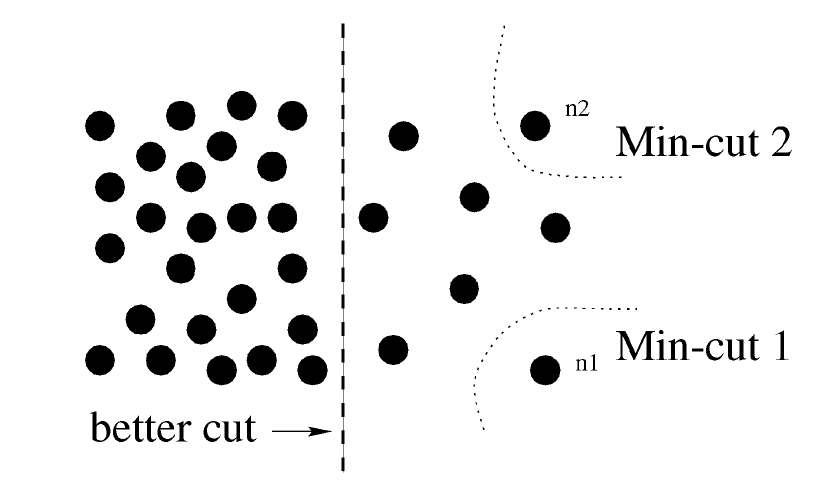
\includegraphics[width=\textwidth]{img/mincutproblem.png}
 \caption{Bad partitioning from \textit{minimum cut} in a particular case \cite{shi_normalized_2000}}
\end{figure}

\paragraph{\textit{Normalised cut}}
To improve this state \cite{shi_normalized_2000} proposed, instead of looking at the total weigh of the edges connecting two groups, to look at a fraction of the total edge connections to all nodes.
This is the \textit{normalised cut}, or \(Ncut\).
The disassociation measure can be formulated as
\[Ncut(A, B) = \frac{cut(A, B)}{assoc(A, V)} + \frac{cut(A, B)}{assoc(B, V)},\]
where \(assoc(A, V) = \sum_{u\in A, t\in V} w(u, t)\), the total connection from the nodes in A to all nodes in the graph.

The goal is still to minimise the \(Ncut\) value, but when \(cut\) is small for isolated pixels, the fraction will be greater because the similarity \(assoc\) between this one pixel and all pixels will be small.
This fraction's denominator will be bigger if the similarity between the selected pixels and all pixels is more important, which makes the fraction smaller.

As it follows, we can define the normalised association measure within groups, such as
\[Nassoc(A, B) = \frac{assoc(A, A)}{assoc(A,V)} + \frac{assoc(B, B)}{assoc(B, V)},\]
where \(assoc(A, A)\) is the total weights of edges inside group \(A\).
This measure quantifies how tightly the nodes of a group are connected to each other.
Deriving the \(Ncut\) equation, we can define that
\[Ncut(A, B) = 2 - Nassoc(A, B).\]

It was shown by \cite{papadimitriou_npcompleteness_1997} and \cite{shi_normalized_2000} that minimising the \(Ncut\) exactly is a NP-complete problem.
However, \cite{shi_normalized_2000} proposes a method to approximate discrete solutions efficiently for the \textit{normalised cut} problem.

Indeed, the proposed algorithm starts by computing the associated similarities for graph \(G = (V, E)\) for the image and store it in the matrices \(K\) and \(D\).

Then, solve \((D-K)x = \lambda Dx\) for the eigenvectors with the smallest eigenvalues.
The way this equation is derived is explicitly shown in \cite{shi_normalized_2000}.
The second-smallest eigenvector is used to bipartition the graph by finding the best splitting point to minimise \(Ncut\), and we see that this approach links to spectral graph theory.
After that, it is possible to use the other eigenvectors to bipartition the graph even more.
Once this is done, we can recursively apply the same algorithm on the segmented groups, stoping when the maximum number of groups is reached or the partitions are not good enough depending on an empirical threshold.

\paragraph{Edge separators and spectral rounding}
Introduced by \cite{tolliver_graph_2006}, edge separators of a graph are created by iteratively reweighting edges until the graph eventually disconnects into groups.
At each iteration, only a small number of eigenvectors are computed to reweight the edges.
This is called spectral rounding by \cite{tolliver_graph_2006} where the detailed algorithm is exposed.

The general idea is an iterative algorithm that reweights edges so it produces a k-way partition.
At the beginning, we define the graph \(G = (V, E, w^0)\) with its initial weights \(w^0\) which can be defined as wanted.
\cite{tolliver_graph_2006} uses the \textit{Intervening Contour} such as described in \cite{shi_normalized_2000} to define the initial weights.
A step of the algorithm is called \textit{SR-Step} and computes \(\{w^{(N)}\}\) of \(N\) weightings such that the graph \(G^N = (V, E, w^N)\) is disconnected into \(k\) components.
These weights are computed according to a valid reweighting scheme, using the eigendecomposition of the graph.
We can observe that partitioning the graph in this manner actually plays on the Cheeger constant and its bounds because we are directly working on the ``bottlenecks" of the graph.
The reweighting function is based on formal fractions, defined by a pair of real numbers \(\frac{a}{b}\) and its value as a real number \(a/b\).
We can define the fractional average as \(\frac{\sum_{i=1}^n a_i}{\sum_{i=1}^n b_i}\) which serves as the basis for defining the inverse fractional reweighting, used as reweighting scheme.
\cite{tolliver_graph_2006} proves that the so-called \textit{SR-Algorithm} converges into a k-way partition by showing, among others, that the \textit{SR-Step} also converges in a finite number of iterations.

\paragraph{Comparison}
This spectral rounding method produces directly discrete solutions, and seems to compare nicely against the \(Ncut\) approximation by producing more human-like results \cite{tolliver_spectral_2006}.
\cite{tolliver_graph_2006} claims that spectral rounding finds better cuts on average than \(Ncut\) based on an empirical evaluation and comparison of the partition entropy.
Anyway, it has been generally accepted that the \(Ncut\) produces better cuts than \textit{minimum cut} for graph partitioning of natural images.

\subsection{3D image processing}

\paragraph{}
In general, \cite{zhang_spectral_2010} sets a very good overview of most variants and applications of spectral processing.
A section is dedicated to mesh Laplacian operators, which are the most commonly used operators for spectral mesh processing, and it summarises that they can be divided into two groups.
First, as studied in \cite{chung_spectral_1997}, \textit{combinatorial mesh Laplacians} which are solely based on the mesh topological information, but still have eigenfunctions that show a remarkable conformity to the mesh geometry.
Second, \textit{geometric mesh Laplacians} encode explicitly the geometric information by a discretisation of the Laplace-Beltrami operator from Riemannian geometry.

Even though both of these categories are noticeably distinct, they can be expressed in a single mathematical definition.
We find again the comparison with the center-surround average when we define that a mesh Laplacian operator takes the difference of the value of a function at a vertex and a weighted average of its neighbour vertices values.

One of the simplest Laplacian definitions is the \textit{first order Laplacian}, where a given vertex only involves the 1-ring neighbours.
A triangle mesh with \(n\) vertices is represented as \(M = (G, P)\) where the graph \(G = (V, E)\) and \(P \in \Real^{n\times 3}\) represents the geometry of the mesh.
For each vertex \(i \in V\), there is an associated position vector denoted \(p_i = [x_i, y_i, z_i]\).
Finally, the set of 1-ring neighbours of \(i\) is formulated as \(N(i) = \{j \in V | (i, j) \in E\}\).


\subsection{Domain decomposition methods}

\paragraph{}
Domain decomposition methods will also be an important topic of this degree project.
Those methods are used to solve problems of linear algebra involing partial differential equations (PDEs).
Functional analysis is used to study PDEs, which is necessary for a numerical approximation.
The discrete equations this is linked to are \(F(u) = b \in \Real^n\), with \(n\) the number of degrees of freedom of the discretisation.
Whether \(F\) is linear or not, solving this problem leads to solving linear systems.

Our main reference will be \cite{dolean_domain_2015} which focuses on the parallel linear iterative solvers for systems of linear equations.
Domain decomposition methods are naturally parallel which is convenient for the current state of processor progress.
Without going into the details, we will focus on Schwarz methods for preconditioning, and mostly iterative Krylov methods, such as the conjugate gradient and GMRES.
The algorithms will be able to find the solution to a Poisson problem \(\Delta \phi = f\), where \(\Delta\) the Laplacian operator and \(f\) a function that is often given.
The goal is to determine \(\phi\) with \(f\) and knowing some boundary value conditions.
These types of problems are well-posed: a solution exists and is unique.

Schwarz algorithms are iterative methods of solving subproblems alternatively in domains \(\Omega_1\) and \(\Omega_2\).
Also important is the use of domain decomposition methods as preconditioners for Krylov methods, which are iterative solvers for linear systems.
We shall also look into direct solvers, for instance the LU factorisation, to understand their limitation on large problems.


\section{Delimitations}

The number of investigated algorithms and variants depend on the pre-study and objectives that make the most sense for 3D images.
It is obviously also limited by the amount of time given to the degree project.
